%____________________________________________________________________________||
\section{Event selection and categorisation}
\label{sec:selection}

This section first outlines the set of ``pre-selection'' requirements
that are common to all signal and control regions, before defining the
selection criteria that are specific to each region.

%%____________________________________________________________________________||
\subsection{Common pre-selection requirements}
\label{sec:preSelection}

The event selection criteria described in this section are common to
all signal and control regions. These selections are summarised in
Table~\ref{tab:pre-selections} and described in further detail below.

\begin{table}[h!]
  \topcaption{Summary of the pre-selection criteria.}
  \label{tab:pre-selections}
  \centering
  \small
  \begin{tabular}{ ll }
    \hline
    \ETmiss quality               & \parbox[t]{12cm}{(Primary Vertex, CSC Beam Halo, HBHE Noise and Isolation,                                 \\
                                    ECAL Endcap SC Noise, ECAL TP, Bad Muon, Bad Charged Hadron)}                                              \\
    Beam halo                     & $0.1 < \mathrm{CHF} < 0.95$ for highest-\Pt jet                                                            \\
    Jet $\mathrm{j}_i$ acceptance & Each jet $\mathrm{j}_i$ that satisfies $\pt^{\mathrm{j}_i} > 40\GeV$ and $\abs{\eta^{\mathrm{j_1}}} < 2.4$ \\
    Jet $\mathrm{j_1}$ acceptance & $\pt^{\mathrm{j_1}} > 100\GeV$                                                                             \\
    Jets below threshold          & $\HTmiss / \ETmiss < 1.25$                                                                                 \\
    Forward jet veto              & Veto events containing a jet satisfying $\pt > 40\GeV$ and $\abs{\eta} > 2.4$                              \\
    Energy sums                   & $\scalht > 200\GeV$ and $\HTmiss > 200\GeV$                                                                \\
    \hline
  \end{tabular}
\end{table}

\subsubsection{MET filters}
\label{sec:metfilters}

A number of beam- and detector-related effects can induce significant
\met. Examples include beam halo, reconstruction failures, spurious
detector noise, or event misreconstruction due to detector
inefficiencies. These events, with large, non-physical values of \met,
are rejected with high efficiency by applying a range of dedicated
vetoes. All ``MET filters'' recommended by the JetMET POG and SUSY PAG
are applied by default in this analysis and listed in
Table~\ref{tab:pre-selections}.

\subsubsection{Charged hadron fraction (CHF) for leading jet}
\label{sec:chf}

In addition to the MET filters, a dedicated filter is applied to
remove beam halo, given that the CSC beam halo filter has been found
to be less efficient during the early Run 2 data-taking period
compared to the previous run.

Beam halo events manifest themselves as single energy deposits in the
calorimeters, which introduces large amounts of ``fake'' \met. This
effect is especially prominent in low-\njet events that satisfy the
signal region requirements, particularly at $\phi$ coordinates of 0
and $\pi$ because of the tendency of halo particles to lie within the
plane of the LHC ring.

Such spurious events are suppressed by requiring at least 10\% of 
the highest-\Pt jet's energy to originate from charged
hadrons. The effectiveness of this charged hadron fraction (CHF)
requirement is demonstrated in Fig.~\ref{fig:leadJetCleaning}
(App.~\ref{app:selection}). 

Further, a requirement of $\mathrm{CHF} < 0.95$ for the highest-\Pt
jet removes events that contain reconstruction failures concerning
muons, which are prevelant in simulated multijet events.

%There is no need for this selection in the control regions, as the
%requirement of well identified physics objects, like muons and photons
%naturally removes spurious events of this kind.

The requirement $0.1 < \mathrm{CHF} < 0.95$ for the highest-\Pt jet
can be regarded as an additional jet ID requirement employed by this
analysis, with efficiency close to unity for real jets and thus not
affecting the signal efficiency significantly.

\subsubsection{Experimental acceptance for jets}
\label{sec:jetsacc}

Jets considered in the analysis are required to satisfy $\PT > 40\gev$
and $|\eta| < 2.4$. The selected jets are used in the calculation of
all jet-based event-level variables, such as \njet, \HT, \mht, and
\alphat (see Sec.~\ref{sec:kine} for their definitions).

The highest-\Pt jet in the event is required to satisfy $\Pt^{\mathrm
  j_1} > 100\gev$. This helps to ensure high trigger efficiencies
while maintaining high efficiency for a broad range of signal models.

Events are classified based on the second highest-\Pt jet, as
described in Sec.~\ref{sec:subleading-jet}.

\subsubsection{The \texorpdfstring{\mht/\met}{HTmiss/ETmiss} variable} 
\label{sec:mhtmet}

The value of \mht is compared to the missing transverse energy
variable, $\met$. Only events that satisfy
$R_{\mathrm{miss}}=\mht/\met < 1.25$ are considered in order to
protect against events containing multiple jets outside the
experimental acceptance (\eg ``below'' the \Pt acceptance) that
contribute significantly to \mht. In the case of the control regions,
in which well-reconstructed, isolated muons and photons are selected,
the $R_{\mathrm{miss}} < 1.25$ requirement is also applied. The \mht
sum does not consider the transverse momentum of the muons or
photon. Hence their transverse momentum vectors are also added to the
\met vector, such that the \mht and \met can be considered on an equal
footing.

\subsubsection{The forward jet veto} 

Events containing jets in the forward region that satisfy the
requirements $\Pt > 40\gev$ and $|\eta|>2.4$ are rejected (regardless
of the identification requirement) to control background contributions
from SM processes such as multijet production, without introducing a
significant reduction in signal acceptance.

\subsubsection{Jet-based energy sums}
\label{sec:energysums}

Events are required to have significant hadronic activity by requiring
$\scalht > 200\GeV$. Despite an increase in both multijet production
cross sections and pileup in Run~2, the lowest \HT threshold is kept
at the same value of the Run~1 analysis~\cite{Chatrchyan:2013lya} in
order to maintain acceptance to DM models or compressed SUSY.

Events are required to have appreciable missing transverse energy by
requiring $\mht>200\gev$. This requirement is applied to events in the
signal and control regions. The threshold differs with respect to the
previous iteration of the analysis, the ICHEP prelimary
result~\cite{CMS-PAS-SUS-16-016}, which used $\HTmiss > 130\GeV$. This
change is motivated through studies that demonstrate a lack of
knowledge of the trigger efficiency in the turn on of the efficiency
curve, prior to the efficiency plateau at $\HTmiss \approx 200\GeV$
(see Sec.~\ref{sec:triggers}).

The \scalht-dependent \alphat thresholds, required to suppress
multijet events as outlined in Sec.~\ref{sec:had-signal}, provide an
effective threshold on \mht in the range 130--200\GeV, via the
relationship in Eq.~(\ref{eq:alphat3}). Hence, the extrapolation from
control to signal region in terms of the \alphat requirement for the
signal region (that is not required for the control regions, see
below) is reduced by the $\mht>200\gev$ requirement.  

\subsection{The signal region}
\label{sec:had-signal}

The event selection criteria specific to the signal region are
described in this section and summarised in
Table~\ref{tab:sr-selections}.

\begin{table}[!h]
  \topcaption{Summary of the event selection criteria for the signal
    region. The criteria are applied in addition to the pre-selection
    requirements listed in Table~\ref{tab:pre-selections}.
  }
  \label{tab:sr-selections}
  \centering
  \begin{tabular}{ ll }
    \hline
    Lepton vetoes              & $\pt > 10\GeV$ and $\abs{\eta} < 2.5$ for isolated muons and electrons                          \\
    Single isolated track veto & $\pt > 10\GeV$  and $\abs{\eta} < 2.5$ for isolated tracks                                      \\
    Photon veto                & $\pt > 25\GeV$ and $\abs{\eta} < 2.5$ for isolated photons                                      \\
    QCD multijet rejection     & $\alphat > \mathrm{threshold}$ (\scalht-dependent, see Table~\ref{tab:alphat-thresholds} below) \\
    QCD multijet rejection     & $\bdphi > 0.5$ ($\njet \geq 2$) or $\bdphimod > 0.5$ ($\njet = 1$)                              \\[0.5ex]
    \hline
  \end{tabular}
\end{table}

\subsubsection{Lepton, photon, and single isolated track vetoes}
\label{sec:vetoes}

Using the identification criteria described in Sec.~\ref{sec:objects},
the following objects are vetoed when selecting events for the
hadronic signal region:
\begin{itemize}
\item muons with $\pt>10\,\mathrm{GeV}$ and $|\eta|<2.5$;
\item electrons with $\pt>10\,\mathrm{GeV}$ and $|\eta|<2.5$;
\item single isolated tracks with $\pt>10\,\mathrm{GeV}$ and
  $|\eta|<2.5$;
\item photons with $\pt>25\,\mathrm{GeV}$ and $|\eta|<2.5$;
\end{itemize}

\subsubsection{\texorpdfstring{\scalht}{HT}-dependent \texorpdfstring{\alphat}{AlphaT} requirements}
\label{sec:HT-AT-selection}

After the pre-selection criteria and the vetoes are applied, the
multijet background is still several orders of magnitude larger than
the typical signal expected from SUSY. Background events from multijet
production populate the region $\alphat \lesssim 0.5$ and therefore
can be rejected with very high efficiency by requiring events to
exhibit an \alphat value above an appropriate
threshold. Sec.~\ref{sec:alphatdef} defines the \alphat variable.

The \alphat thresholds are also chosen in order to ensure a trigger
efficiency close to unity in all the bins. More details on the trigger
strategy can be found in Sec.~\ref{sec:triggers}.

\begin{table}[h!]
  \caption{\alphat thresholds versus
    lower bound of \scalht bin. For all \HT bins satisfying $\HT >
    900\gev$, no \alphat cut is applied, and similarly for events with
     $\njet = 1$ (``monojet'' events, see
    Sec.~\ref{sec:subleading-jet}). Also
    shown is the flat \bdphi requirement
    (Sec.~\ref{sec:bdphi-selection}).}   
  \label{tab:alphat-thresholds}
  \centering
  \begin{tabular}{ lcccccccc }
    \hline
    \scalht [GeV]     & 200--250 & 250--300 & 300--350 & 350--400 & 400--900 & 900--1200 & $>$1200 \\
    \alphat threshold & 0.65     & 0.60     & 0.55     & 0.53     & 0.52     & (none)    & (none)  \\
    \bdphi threshold  & 0.5      & 0.5      & 0.5      & 0.5      & 0.5      & 0.5       & 0.5     \\
    \hline
  \end{tabular}
\end{table}

Table~\ref{tab:alphat-thresholds} summarises the \alphat thresholds
for each \HT bin. The \alphat threshold is dependent only on \HT and
not on \njet nor \nb that are used to define the event categories. No
\alphat cut is applied for events satisfying $\njet = 1$ (``monojet''
events, see Sec.~\ref{sec:subleading-jet}), as the variable is defined
only for $\njet \geq 2$. Further, no requirement is made for events
satisfying $\scalht > 1200\GeV$.

\subsubsection{\texorpdfstring{\bdphi}{biased dPhi} requirement} 
\label{sec:bdphi-selection}

Candidate signal events with two or more jets are accepted only if
they satisfy $\bdphi > 0.5$. This threshold is independent of \scalht,
unlike the \alphat requirement described above, as summarised in
Table~\ref{tab:alphat-thresholds}. In the case of events satisfying
$\njet = 1$ (``monojet'' events, see Sec.~\ref{sec:subleading-jet}),
the requirement $\bdphimod > 0.5$ must be satisfied. The definitions
of \bdphi and \bdphimod can be found in Sec.~\ref{sec:bdphi-def}. 

\subsection{The control regions}
\label{sec:control-region-selection}

The event selection criteria specific to the various control regions
are described in this section and summarised in
Table~\ref{tab:cr-selections}.

\begin{table}[!h]
  \topcaption{Summary of the event selection criteria for the signal
    region. The criteria are applied in addition to the pre-selection
    requirements listed in Table~\ref{tab:pre-selections}. One of the
    lepton or photon vetoes in Table~\ref{tab:sr-selections} are
    inverted to define each lepton- or photon-based control
    region. Additional kinematic requirements are made to ensure the
    samples are signal-depleted (and multijet-depleted in
    the case of the muon and photon samples). 
  }
  \label{tab:cr-selections}
  \centering
  \small
  \begin{tabular}{ ll }
    \hline
    \mj      & 
    1$\mu$ with $\pt > 30\GeV$, $\abs{\eta} < 2.1$,
    $I^{\mu}_\text{rel} < 0.1$,
    $\Delta R(\mu,\mathrm{j}_i) > 0.5$,
    $30 < m_\mathrm{T}(\ptvec^\mu,\ptvecmiss) < 125\GeV$ \\[0.5ex]
    \mmj     & 
    2$\mu$ with $\pt > 30\GeV$, $\abs{\eta} < 2.1$,
    $I^{\mu}_\text{rel} < 0.1$,
    $\Delta R(\mu_{1,2},\mathrm{j}_i) > 0.5$,
    $ \abs{m_{\mu\mu} - m_\text{Z}} < 25\GeV$            \\[0.5ex]
    \gj      & 
    1$\gamma$ with $\pt > 200\GeV$, $\abs{\eta} < 1.45$,
    $\Delta R(\gamma,\mathrm{j}_i) > 1.0$                \\[0.5ex]
    Multijet & SR selection (Table~\ref{tab:sr-selections}) + inverted $\HTmiss/\ETmiss$ and $\bdphi$ requirements (Table~\ref{tab:qcd_sidebands}) \\
    \hline
  \end{tabular}
\end{table}

\subsubsection{The \texorpdfstring{\mj}{muon + jets} control sample}
\label{sec:mucontrolSelection}

The selection criteria for the \mj sample are chosen to identify W
bosons decaying to a muon and a neutrino in the phase-space of the
signal. In order to select events containing W bosons, exactly one
tight isolated muon (defined in Sec.~\ref{sec:muon-id}) within an
acceptance of \PT $>$ 30 \gev and $|\eta| <$ 2.1 is required. The
muons is removed from the event while computing all jet-based
quantities, like \mht and \alphat, as well as \ETmiss. The transverse
mass of the W candidate must satisfy $30 < \mt(\mu,\pfmet) < 125\gev$.
This cut is also effective in reducing potential signal contamination
for final states with leptons.  Events are vetoed if $\Delta
R(\mu,\textrm{jet}) < 0.5$ for at least one jet.

Events are vetoed if well-reconstructed, isolated electrons and
photons, defined in Sec.~\ref{sec:objects}, are found to be within the
acceptances defined in Sec.~\ref{sec:vetoes}. Similarly, events
containing single isolated tracks (not associated with the identified
muon) are also vetoed according to the object and acceptance
definitions found in Secs.~\ref{sec:objects}
and~\ref{sec:vetoes}. Hence the vetoes mirror exactly those used in
the signal region, except for the selected muon.

\subsubsection{The \texorpdfstring{\mmj}{di-muon + jets} control sample}
\label{sec:mumucontrolSelection}

The selection criteria are identical to those for the \mj sample, with
the following exceptions that are tuned to identify Z bosons decaying
to two muons in the kinematic phase space of the signal region.  In
order to select an event sample containing Z bosons, exactly two tight
isolated muons (defined in Sec.~\ref{sec:muon-id}) within an
acceptance of $\Pt > 30\gev$ and $|\eta| < 2.1$ are required. The two
muons are required to have opposite electric charge and the invariant
mass of the two muons must satisfy $m_{Z} - 25 < M_{\mu_1\mu_2} <
m_{Z} +25$.  Events are vetoed if $\Delta R(\mu,\textrm{jet}) < 0.5$
is satisfied, running over all muons and all jets.

Events are vetoed if well-reconstructed, isolated electrons and
photons, defined in Sec.~\ref{sec:objects}, are found to be within the
acceptances defined in Sec.~\ref{sec:vetoes}. Similarly, events
containing single isolated tracks (not associated with the identified
muons) are also vetoed according to the object and acceptance
definitions found in Secs.~\ref{sec:objects}
and~\ref{sec:vetoes}. Hence the vetoes mirror exactly those used in
the signal region, except for the selected muons.

\subsubsection{The \texorpdfstring{\gj}{photon + jets} control sample}
\label{sec:photoncontrolSelection}

Even though the \gj sample is no longer used in the likelihood model
of the analysis, it is still used in cross check studies and so is
described here.

The \gj sample is defined by requiring exactly one photon (defined in
Sec.~\ref{sec:photon-id}) satisfying tight isolation criteria and
within an acceptance of $\pt > 200\gev$ (limited by trigger
requirements) and $|\eta| < 1.45$. Furthermore, events are vetoed if
$\Delta R(\gamma,\textrm{jet}) < 1.0$ is satisfied for any jet.

Events are vetoed if well-reconstructed, isolated muons and electrons,
defined in Sec.~\ref{sec:objects}, are found to be within the
acceptances defined in Sec.~\ref{sec:vetoes}. Similarly, events
containing single isolated tracks are also vetoed according to the
object and acceptance definitions found in Secs.~\ref{sec:objects}
and~\ref{sec:vetoes}. Hence the vetoes mirror exactly those used in
the signal region, except for the selected photon.

\subsubsection{The multijet-enriched control region}
\label{sec:multijetcontrolSelection}

QCD multijet-enriched event samples are defined by the application of
the same event selection criteria used to define the signal region,
summarised in Sec.~\ref{sec:had-signal}, except for the inversion of
one or both of the following (signal region) requirements: $\mht/\met
> 1.25$ and/or $\bdphi > 0.5$. An upper bound for the $\mht/\met$
sideband is applied: $1.25 < \mht/\met < 3.0$. A lower bound for the
$\bdphi$ sideband is applied: $0.2 < \bdphi < 0.5$. Further details
can be found in Sec.~\ref{sec:qcd}.

Events are vetoed if well-reconstructed, isolated muons, electrons, or
photons, defined in Sec.~\ref{sec:objects}, are found to be within the
acceptances defined in Sec.~\ref{sec:vetoes}. Similarly, events
containing single isolated tracks are also vetoed according to the
object and acceptance definitions found in Secs.~\ref{sec:objects}
and~\ref{sec:vetoes}. Hence the vetoes mirror exactly those used in
the signal region.

\subsection{Event categorisation}
\label{sec:event-categorisation}

This section summarises how the events are categorised in the signal
and control regions, from the point of view of signal extraction
(using the likelihood fit) and validation of the simulation modelling
of variables in which extrapolations are performed.

\subsubsection{Discriminating variables}

\begin{table}[!h]
  \topcaption{Summary of the variables used to categorise events in
    the likelihood model for the signal and each control region. Also
    shown are the variables used for modelling (\ie validation)
    studies. $\dagger$The \mmj sample performs a limited extrapolation
    in \nb, as described in the text below and in
    Sec.~\ref{sec:nb-categorisation}. 
  }
  \label{tab:cr-categorisation}
  \centering
  \begin{tabular}{ lll }
    \hline
    Sample   & Used in likelihood model     & Used for modelling (\ie validation) studies \\ 
    \hline
    \mj      & \njet, \scalht, \nb          & \HTmiss                                     \\
    \mmj     & \njet, \scalht, \nb$\dagger$ & \nb, \HTmiss                                \\
    Multijet & \njet, \scalht               & \nb, \HTmiss                                \\
    \gj      & --                           & \njet, \scalht, \nb, \HTmiss                \\
    \hline
  \end{tabular}
\end{table}

The event categorisation used by the likelihood model differs
according to the sample. Events in the signal region are categorised
according to \njet, \nb, \scalht, and \HTmiss. 

The \mj events are categorised identically according to \njet, \nb,
and \scalht. The modelling of \HTmiss is checked in the \mj sample.

Events in the \mmj and multijet-enriched control regions are also
categorised indentically according to \njet and \scalht. However, for
the \mmj events, two \nb categories are employed, $\nb = 0$ and $\nb
\geq 1$, and an extrapolation in \nb is performed for the region $\nb
\geq 1$. The simulation modelling of the \nb and \mht variables are
checked with both samples.

The \gj sample is not used at all in the likelihood model to estimate
the SM backgrounds in the signal region, but the \gj sample is used to
check the modelling of all variables, \njet, \nb, \scalht, and
\HTmiss. 

This information is summarised in Table~\ref{tab:cr-categorisation}.

\subsubsection{Event categorisation by subleading jet \texorpdfstring{\Pt}{pT}}
\label{sec:subleading-jet}

Events are categorised according to the ``topology'' exhibited by the
two leading jets in the event. The topology is defined in terms of the
\Pt of the subleading jet, $\pt^{\mathrm{j_2}}$, as summarised in
Table~\ref{tab:subleading-jet}.

\begin{table}[h!]
  \topcaption{Summary of topologies, based on \Pt requirement for the
    subleading jet.} 
  \label{tab:subleading-jet}
  \centering
  \begin{tabular}{ lr }
    \hline
    Monojet    & $\pt^{\mathrm{j_2}} < \phantom{1}40\GeV$       \\
    Asymmetric & $40 < \pt^{\mathrm{j_2}} < 100\GeV$ \\
    Symmetric  & $\pt^{\mathrm{j_2}} > 100\GeV$      \\
    \hline
  \end{tabular}
\end{table}

If the subleading jet is outside the experimental acceptance (\ie
$\Pt^{\mathrm j_2} < 40\gev$), the event is assigned to the
``monojet'' topology. If $40 < \Pt^{\mathrm j_2} < 100\gev$, the event
is assigned to the ``asymmetric'' topology. The asymmetric and monojet
topologies have been added to the analysis to help improve acceptance
to a range of DM models and compressed SUSY.

In the case that a second leading jet satisfies $\PT > 100\gev$, the
event is categorised as exhibiting a ``symmetric'' topology. This
raised threshold helps to improve the S/B for a wide range of models
involving pair production with respect to SM processes, such as V +
jets production.

\subsubsection{Event categorisation by \texorpdfstring{\njet}{Njet}}
\label{sec:njet-categorisation}

\begin{table}[h!]
  \topcaption{Summary of \njet categorisation (including topology)
    used in this analysis. The character labels used throughout
    the documentation are also listed.}
  \label{tab:njet-binning}
  \centering
  \begin{tabular}{ lll }
    \hline
    \njet   & Topology   & Label \\ 
    \hline
    1       & Monojet    & eq1j  \\
    $\geq$2 & Asymmetric & ge2a  \\
    2       & Symmetric  & eq2j  \\
    3       & Symmetric  & eq3j  \\
    4       & Symmetric  & eq4j  \\
    5       & Symmetric  & eq5j  \\
    $\geq$6 & Symmetric  & ge6j  \\
    \hline
  \end{tabular}
\end{table}

Table~\ref{tab:njet-binning} shows the categorisation of events,
according to \njet and topology, used in this analysis. Seven ``\njet
bins'' (categories in \njet and topology) are employed, and this
scheme is used identically in all signal and control regions.

\subsubsection{Event categorisation by \texorpdfstring{\scalht}{HT}}
\label{sec:ht-categorisation}

In the control regions, up to eleven \scalht bins are employed with
variable bin widths:
\begin{itemize}
\item 4 bins of width 50\GeV in the region 200--400\GeV;
\item 2 bins of width 100\GeV for 400--600\GeV; 
\item 4 bins of width 150\GeV for 600--1200\GeV;
\item and a final open bin, $\scalht > 1200\GeV$. 
\end{itemize}

For the signal region, the predictions derived from the eleven bins in
\scalht in each control region are aggregated to reduce the number of
\scalht bins in the signal region to just five: 
\begin{itemize}
\item 200--400, 
\item 400--600,
\item 600--900, 
\item 900--1200, 
\item $>$1200\GeV.  
\end{itemize}

The aggregation scheme preserves information on the \scalht shape in
data from the control region while reducing the number of bins in the
signal region. The aggregation scheme is incorporated into the
likelihood model and preserves all assumptions on systematic
uncertainties and any correlated behaviour across bins. 

\begin{table}[!h]
  \topcaption{Summary of the \scalht [GeV] binning schemes used by the
    control and signal regions, and the aggregation scheme. The
    horizontal lines delineate the aggregation regions.
  }  
  \label{tab:ht-aggr}
  \centering
  \begin{tabular}{ cc }
    \hline
    Control regions  & Signal region       \\
    (Nominal scheme) & (Aggregated scheme) \\
    \hline
    200--250         & 200--400            \\
    250--300         & 200--400            \\
    300--350         & 200--400            \\
    350--400         & 200--400            \\
    \hline
    400--500         & 400--600            \\
    500--600         & 400--600            \\
    \hline
    600--750         & 600--900            \\
    750--900         & 600--900            \\
    \hline
    900--1050        & 900--1200           \\
    1050--1200       & 900--1200           \\
    \hline
    $>$1200          & $>$1200             \\
    \hline
  \end{tabular}
\end{table}

The nominal and aggregated \scalht binning schemes, for the control
and signal regions respectively, are summarised in 
Table~\ref{tab:ht-aggr}.

The \scalht bins in the signal region, and the corresponding \scalht
bins in each control region, are merged or dropped in case of
restricted phase space or low event counts. In the case of low values
of \scalht and high values of \njet, the phase space is nonphysical or
restricted, and so the \scalht bins are not used in the analysis. The
lower bound of the first \scalht bin as a function of \njet is
summarised in Table~\ref{tab:sr-ht-binning}. The merging of bins at
high \scalht is depedent on both \njet and \nb, and is summarised in
Table~\ref{tab:sr-binning} in Sec.~\ref{sec:nb-categorisation}. 

\begin{table}[!h]
  \topcaption{Summary of the lower bound of the first \scalht bin as a
    function of \njet category. }
  \label{tab:sr-ht-binning}
  \centering
  \begin{tabular}{ lccccccc }
    \hline
    \njet         & eq1j & ge2a & eq2j & eq3j & eq4j & eq5j & ge6j \\
    \scalht [GeV] & 200  & 200  & 200  & 200  & 400  & 400  & 400  \\
    \hline
  \end{tabular}
\end{table}

\subsubsection{Event categorisation by  \texorpdfstring{\nb}{Nb}}
\label{sec:nb-categorisation}

Event categorisation by \nb depends on \njet and \scalht, and is
chosen based on data event counts in the \mj and \mmj samples. The
binning in \nb is bounded from above by \njet and determined based on
data event counts in the \mj control region. The event counts in the
\mmj sample are categorised according to counts in (\njet, \scalht,
$\nb = 0$) and (\njet, \scalht, $\nb \geq 1$), with the single
exception of ($\njet = 1$, $\scalht > 900$, $\nb \geq 0$), for which
the \nb dimension is completely collapsed. 

Figure~\ref{fig:cr-counts} (in Appendix~\ref{app:selection}) shows the
event counts as a function of \njet, \nb, and \scalht in \mj, \mmj,
and \gj samples. The binning utilised by the analysis aims to maintain
sufficiently high counts to operate mainly in the Gaussian regime, and
is summarised in Table~\ref{tab:sr-binning}.

\begin{table}[!h]
  \topcaption{Summary of the lower bound of the final open \scalht bin
    [GeV] as a function of \njet and \nb. The lower bound of the first
    \scalht bin is summarised in Table~\ref{tab:sr-ht-binning}. The
    dashes (--) signify (\njet, \nb) bins that are not possible or
    used.
  }
  \label{tab:sr-binning}
  \centering
  \begin{tabular}{ lccccc }
    \hline
    $\njet\, / \,\nb$ & 0    & 1    & 2    & 3    & $\geq$4 \\
    \hline
    eq1j              & 900  & 900  & --   & --   & --      \\ 
    ge2a              & 900  & 900  & 900  & 600  & --      \\ 
    eq2j              & 1200 & 1200 & 900  & --   & --      \\ 
    eq3j              & 1200 & 1200 & 1200 & 900  & --      \\ 
    eq4j              & 1200 & 1200 & 1200 & 900  & --      \\ 
    eq5j              & 1200 & 1200 & 1200 & 900  & 400     \\ 
    ge6j              & 1200 & 1200 & 1200 & 1200 & 400     \\ 
    \hline
  \end{tabular}
\end{table}

\subsubsection{Event categorisation by \texorpdfstring{\HTmiss}{HTmiss}}
\label{sec:htmiss-categorisation}

Events in the signal region are additionally categorised according to
\HTmiss. ``Templates'' determined per (\njet, \scalht, \nb) bin are
used. The templates are determined from simulation and extensively
validated in the data control regions. Uncertainties in these
templates are also determined for a range of uncertainty sources as
well as from cross checks in data.

\HTmiss is at most divided into four bins with boundaries at 200--400,
400--600, 600--900, and $\ge$900\GeV.  As such, the \HTmiss binning scheme
aligns with the \scalht bins.

Finally, the aforementioned \HTmiss binning scheme is modified to
account for finite-size simulation samples. To ensure a sufficiently
populated \HTmiss template can be constructed from simulated events,
at least 500 unweighted simulation events are required in each (\njet,
\scalht, \MHT) bin, inclusive with respect to \nb. Adjacent \HTmiss
bins for each template are merged until this requirement is satisfied.

\begin{table}[!h]
  \topcaption{Summary of the lower bound of the final \HTmiss bin
    [GeV] as a function of \njet and \scalht (signal region,
    aggregated scheme). The lower bound of the first \scalht bin is
    summarised in Table~\ref{tab:sr-ht-binning}. The dashes (--)
    signify (\njet, \nb) bins that are not possible or used.  
  }
  \label{tab:mht-binning}
  \centering
  \begin{tabular}{ lccccc }
    \hline
    $\njet\, / \,\scalht$ [GeV] & 200--400 & 400--600 & 600--900 & 900--1200 & $>$1200 \\
    \hline
    eq1j                        & 900      & 900      & --       & --        & --      \\ 
    ge2a                        & 900      & 900      & 900      & 600       & --      \\ 
    eq2j                        & 900      & 900      & 900      & --        & --      \\ 
    eq3j                        & 900      & 900      & 900      & 900       & --      \\ 
    eq4j                        & 900      & 900      & 900      & 900       & --      \\ 
    eq5j                        & 900      & 900      & 900      & 900       & 400     \\ 
    ge6j                        & 900      & 900      & 900      & 900       & 400     \\ 
    \hline
  \end{tabular}
\end{table}

\subsubsection{Summary of event categorisation}
\label{sec:binning-summary}

The binning strategy is summarised as follows: 
\begin{itemize}
\item In the signal and all control regions, seven \njet categories
  are employed (Table~\ref{tab:njet-binning}). 
\item In the control regions, up to eleven \scalht categories are
  used (Tables~\ref{tab:ht-aggr}, \ref{tab:sr-ht-binning}, and
  \ref{tab:sr-binning}).  
\item In the signal and all control regions, up to five \nb categories
  are used.
\item In the signal region, up to four \HTmiss categories are used.
\item The number of (\njet, \scalht) categories in each control region
  is 61.
\item The number of (\njet, \scalht, \nb) categories in the \mj
  control region is 207.
\item The number of (\njet, \scalht, \nb) categories in the \mmj
  control region is 121.
\item An extrapolation in \nb is performed from the \mmj (for the
  region $\nb \geq 1$ only) and multijet control regions.
\item An extrapolation in \HTmiss is performed from all control regions.
\end{itemize}
In the signal region, after aggregation across \scalht bins: 
\begin{itemize}
\item There are up to five \scalht categories.
\item The number of (\njet, \scalht) cateogories is 30.
\item the number of (\njet, \scalht, \nb) categories is 104.
\item the total number of (\njet, \scalht, \nb, \HTmiss) categories is
  276. 
\end{itemize}

The total number of measurements used in the binned likelihood fit,
which includes the signal, \mj, and \mmj control regions, is 276 + 204
+ 121 = 601. (The multijet background estimates are determined in a
separate fit.) Further details can be found in
Sec.~\ref{sec:likelihood}.

\subsection{Breakdown of SM backgrounds in signal region}%and control regions}
\label{sec:smbreakdown}

Figure~\ref{fig:breakdownmc} summarises the breakdown of SM
backgrounds, categorised as lost lepton, \znunuj, or multijet, in the
signal region as determined from simulation, following the application
of the event selection criteria detailed in Sec.~\ref{sec:had-signal}
and categorised according to the scheme outlined in
Sec.~\ref{sec:event-categorisation}.

\begin{figure}[h!]
  \centering
  \caption{Breakdown of SM backgrounds in the signal region as
    determined from simulation.}
  \label{fig:breakdownmc}
  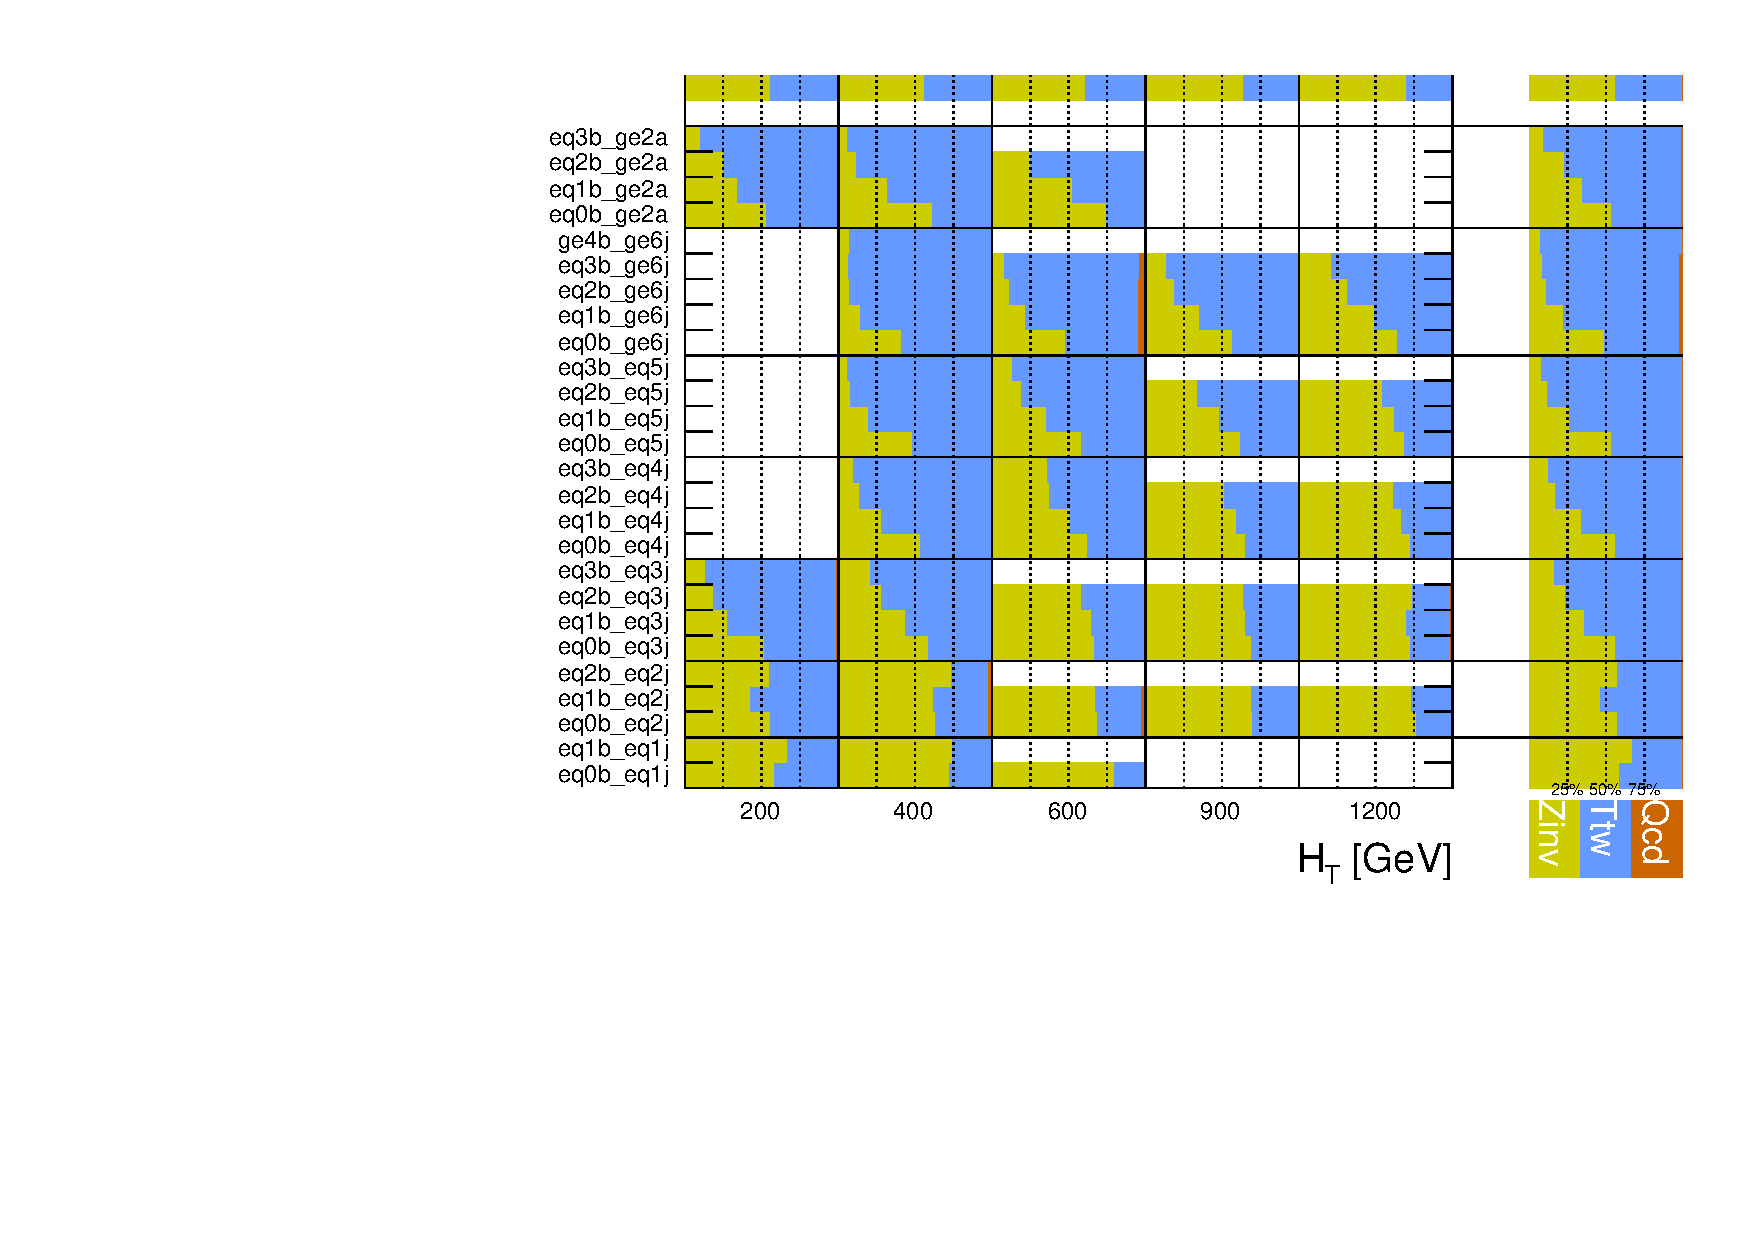
\includegraphics[width=0.8\linewidth]{figures/results/36invfb/breakdown/prefit/Signal_sample_composition.pdf}\\
\end{figure}
